\documentclass[12]{article}
\usepackage{prettyref}
\usepackage[left=2cm,right=2cm,top=2cm,bottom=2cm]{geometry}
\usepackage{graphicx}
\usepackage{amsmath, amssymb}
\usepackage{mathtools}
\usepackage{physics}
\usepackage{textcomp}
\usepackage{float}
\usepackage{hyperref}
\hypersetup{
    colorlinks=true,
    linkcolor=blue,
    filecolor=magenta,      
    urlcolor=cyan,
}
\begin{document}
\begin{center}
\begin{Huge}
RESULTS-Original
\end{Huge}
\end{center}
%\chapter{Results}\label{ch:O}
\section{Second order}
Since Suzuki-Trotter product formula is only an approximation to solve the time dependent Schr{\"o}dinger equation, the error involved depends on the time interval t - the time step at which the evolution is computed (equation \ref{eq:n20}). 

Thus, for checking if the evolution using the Suzuki-Trotter product formula is indeed second order, the dependence of the error should be verified to be quadratic in t, in accordance with equation (\ref{eq:n21}). 
\begin{figure}[H]
\centering 
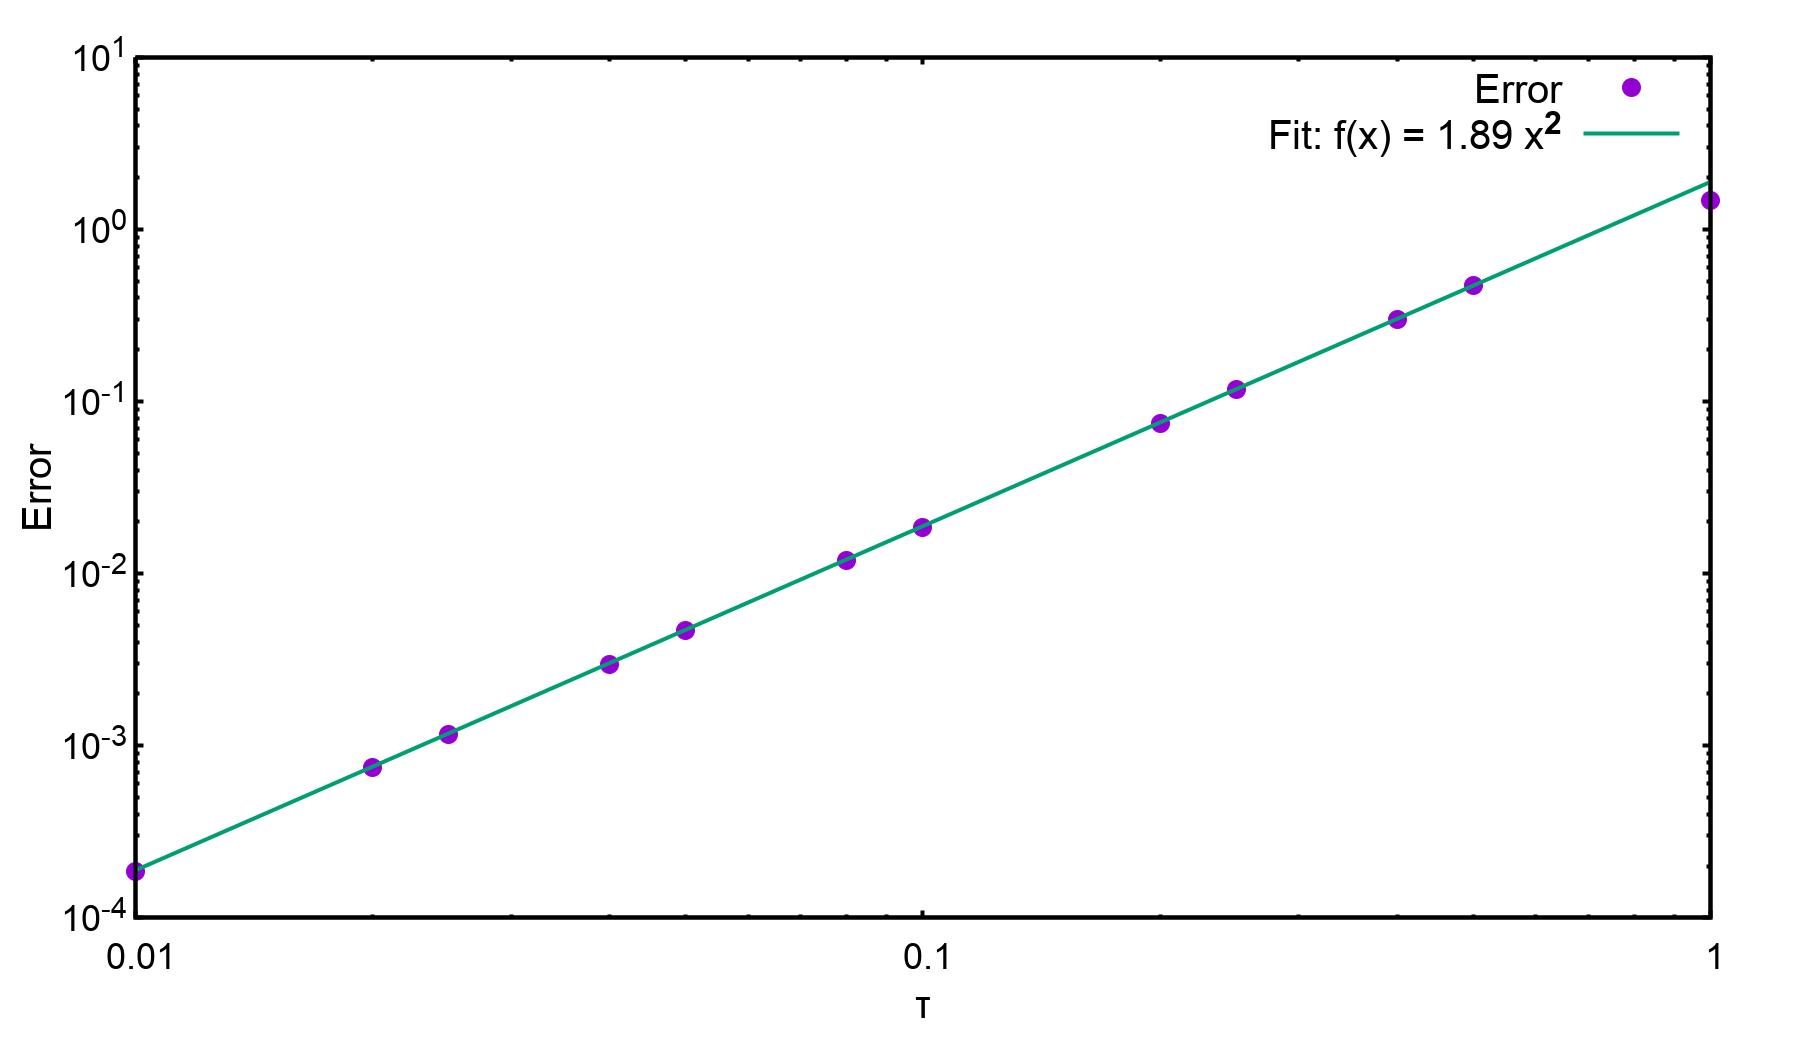
\includegraphics[scale=0.3]{Error.png}
\caption{The error in Suzuki-Trotter formula relative to the full diagonalization method. The involved error grows quadratically in t.}
\label{fig:o1}
\end{figure}
Since the dependence of error on t can be approximated well by a straight line in the log scale, as shown in figure (\ref{fig:o1}), the simulation implementing TDSE can be trusted to be following second order Suzuki-Trotter product formula.

For the course of this thesis, we worked with 8 spin and 12 spin 2-SAT problems. The first set had 91 unique problems, while the second set had 1000 such problems. All the problems had a predetermined unique ground state, and only one avoided crossing between the ground and the first excited state. The success probability was then obtained by calculating the overlap between the known ground state and the final state resulting from the code performing product evolution. Furthermore, for determining the energy spectra for specific problems, the exact diagonalization method was employed.

This chapter focusses on the results obtained for original annealing Hamiltonian, that is in the absence of any triggers. 


For every problem belonging to both the sets, three annealing times were chosen to calculate the success probability. These correspond to $T_A \in \{ 10,100,1000 \}$. For a given $T_A$, the resulting probability is a function of the minimum energy gap, $\Delta$, between the ground and the first excited state. The smaller the value of the minimum energy gap, the smaller is the success probability expected to be, for an adiabatic sweep through the Hamiltonian. Thus, the hardness of a problem can be estimated by its minimum energy gap.\\


As the first example, considered here is a 12-spin problem with high success probability, $p=0.994433$ for $T_A=100$. Figure (\ref{fig:o2}), shows the energy spectrum for this problem. The minimum energy gap, $\Delta$ was found to be 0.440730 in this case.  Also plotted in the figure are the instantaneous energy values obtained from annealing with the above-mentioned annealing times.
\begin{figure}[H]
\centering 
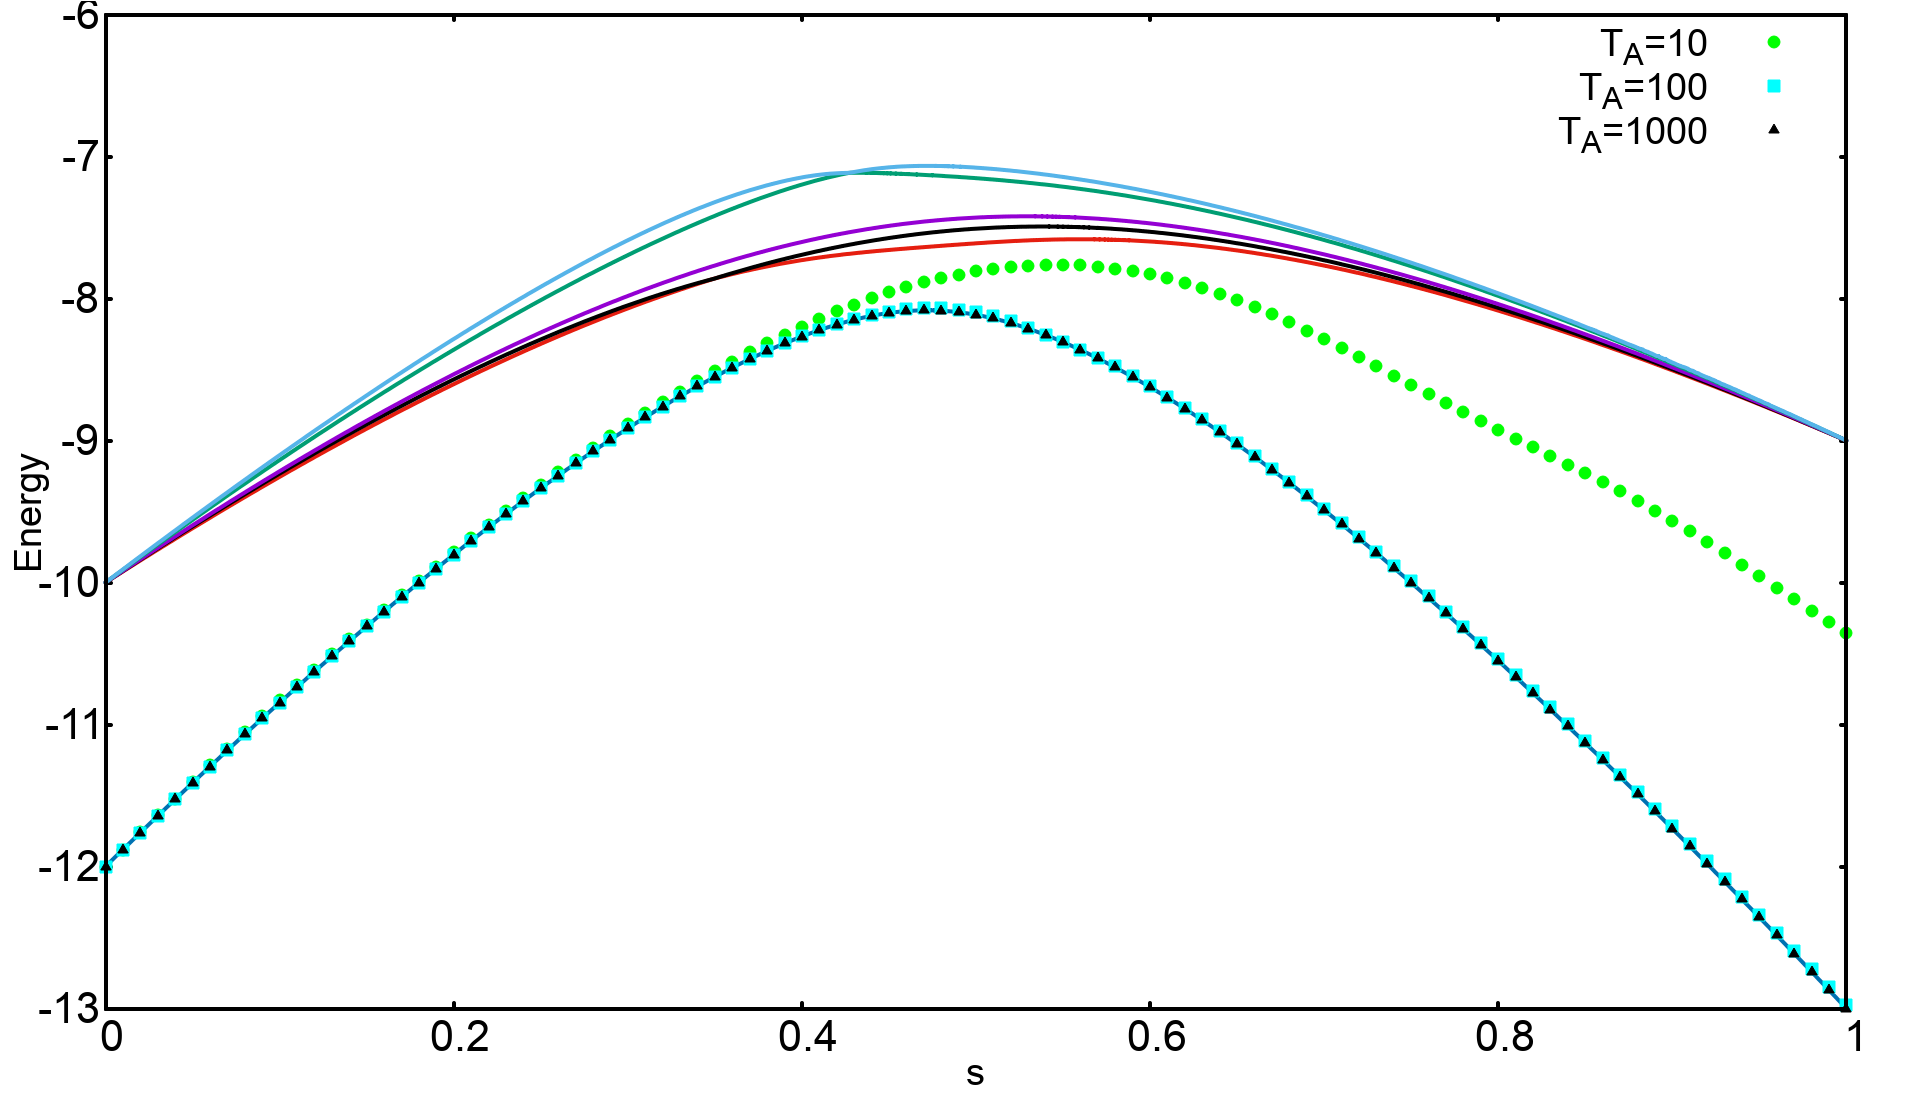
\includegraphics[scale=0.3]{733_s12_O.png}
\caption{The energy spectrum for the selected problem, with instantaneous energy values corresponding to three annealing times. For $T_A$=100, $p$ was found to be 0.994433, while $\Delta=0.440730.$}
\label{fig:o2}
\end{figure}

As expected, the overlap of the final state with the ground state of the problem Hamiltonian increases on increasing the total annealing time in figure (\ref{fig:o2}).\\

Secondly, a 12-spin problem with small success probability, $p= $0.014638 at $T_A=100$, was chosen. Figure (\ref{fig:o3}) shows the energy spectrum and the instantaneous energy values corresponding to three annealing times, for this problem. It should be noted, that the minimum gap in figure (\ref{fig:o3}) has decreased, to $\Delta = 0.031213$, in comparison to that in figure (\ref{fig:o2}). This explains the decrease in success probability for same annealing time.\\
\begin{figure}[H]
\centering 
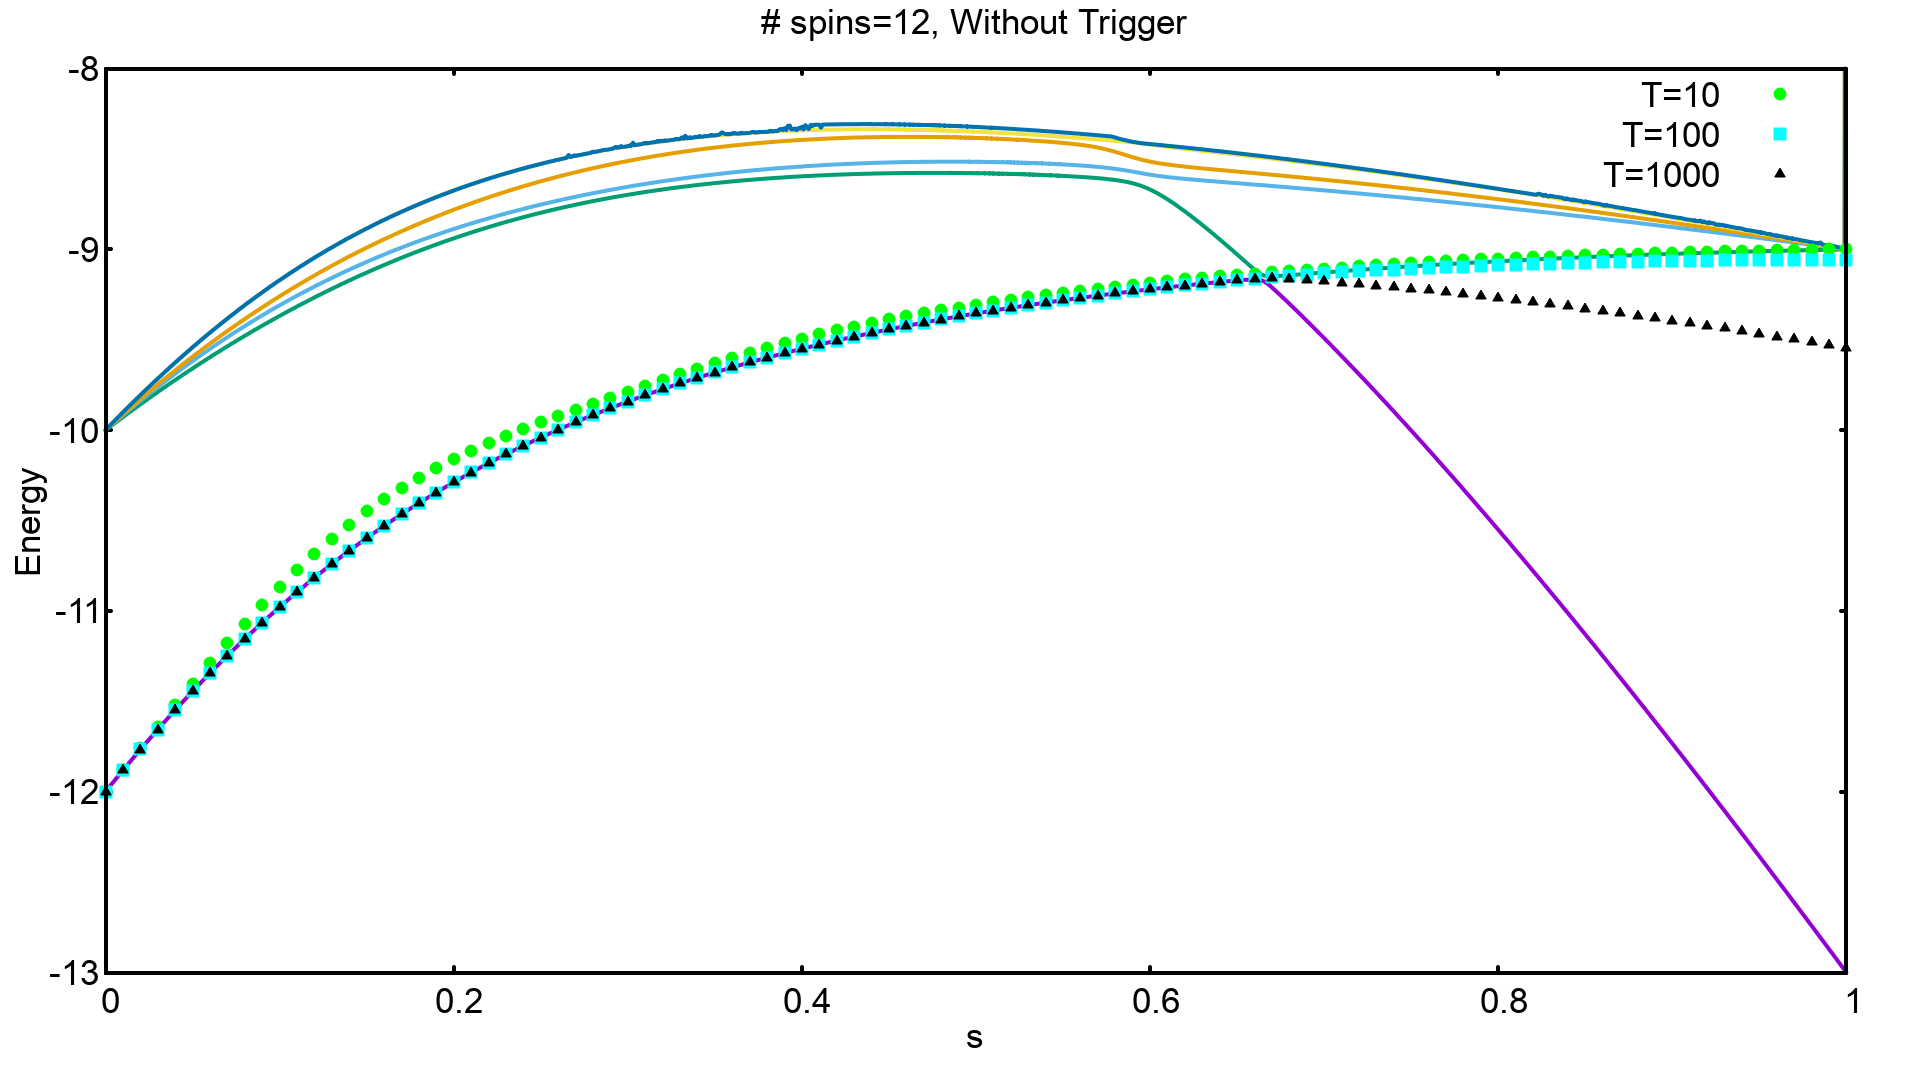
\includegraphics[scale=0.3]{950_s12_O.png}
\caption{The energy spectrum for the selected problem, with instantaneous energy values corresponding to three annealing times. For $T_A$=100, $p$ was found to be 0.014638, while $\Delta=0.031213.$}
\label{fig:o3}
\end{figure}


As the third case, another 12-spin problem with an intermediate success probability of $p=0.519862$ at $T_A= 100$ has been considered. For this case too, the energy spectrum and the instantaneous energy values for the three annealing times was determined, as is shown in figure (\ref{fig:o4}). As expected, the value of minimum gap is $\Delta=0.157325$ for this problem, which lies in between the above two cases. 
\begin{figure}[H]
\centering 
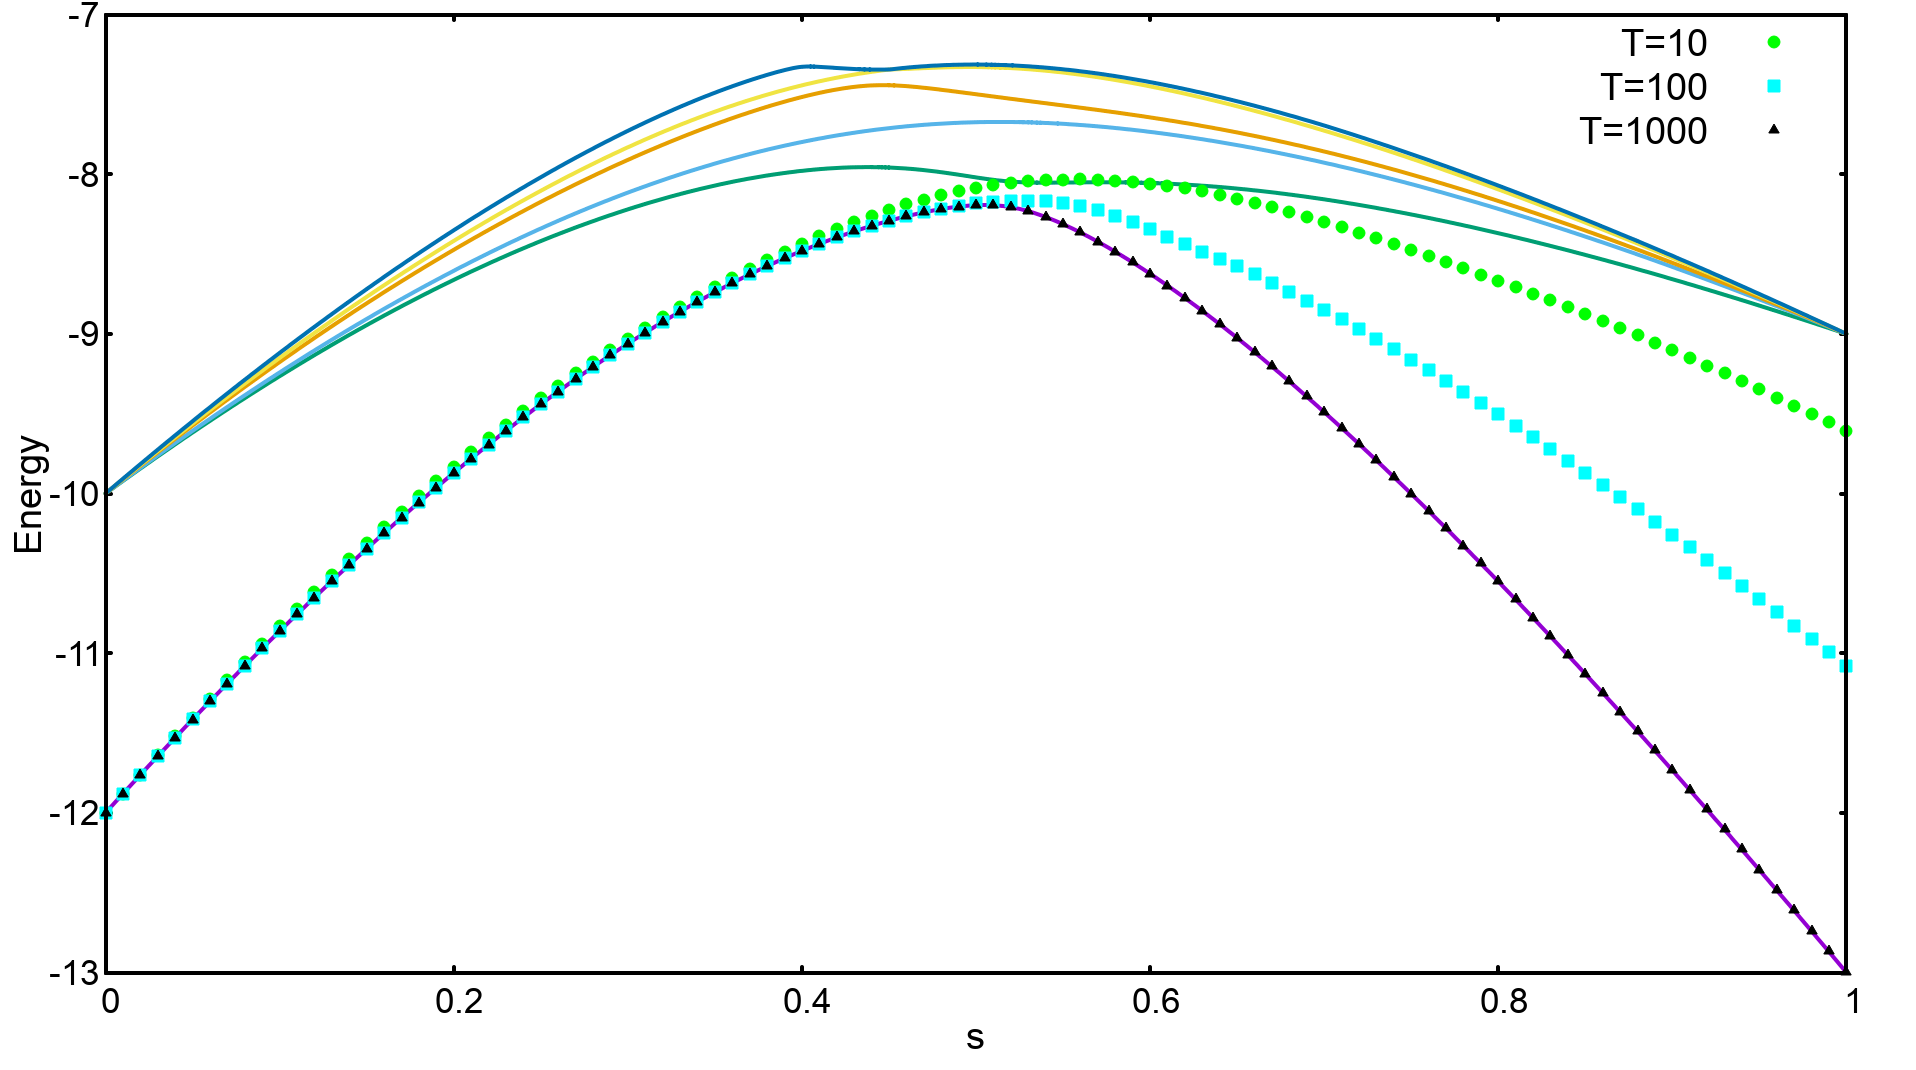
\includegraphics[scale=0.3]{528_s12_O.png}
\caption{The energy spectrum for the selected problem, with instantaneous energy values corresponding to three annealing times. For $T_A$=100, $p$ was found to be 0.519862, while $\Delta=0.157325.$}
\label{fig:o4}
\end{figure}

\newpage
A similar trend was also obtained for 8-spin problems, where the cases with high success probability also were the ones with comparatively larger minimum energy gaps than cases with low success probability.  As examples, three cases, with relatively large, small and intermediate success probabilities were chosen. The respective plots for their energy spectrum and the instantaneous energy values for the different annealing times are shown in the following figures (\ref{fig:o5}, \ref{fig:o6}, \ref{fig:o7}).

The main feature of difference between the 12-spin and 8-spin problems is that the minimum energy gaps of the 8-spin problems are evidently larger than those of 12-spin problems. This can be understood with the help of equation (\ref(eq:n8)), where the minimum gap is expected to close exponentially with increasing N. Even the gap corresponding to the case with smallest success probability in 8-spin problems (the smallest energy gap amongst 91 8-spin problems, $\Delta=0.472494$) is still larger than the the gap corresponding to the case with largest success probability in 12-spin problems (the largest energy gap amongst 1000 12-spin problems, $\Delta=0.440730$). Therefore, even an annealing time of $T_A=100$ yields a large success probability for almost all the cases. 
\begin{figure}[H]
\centering 
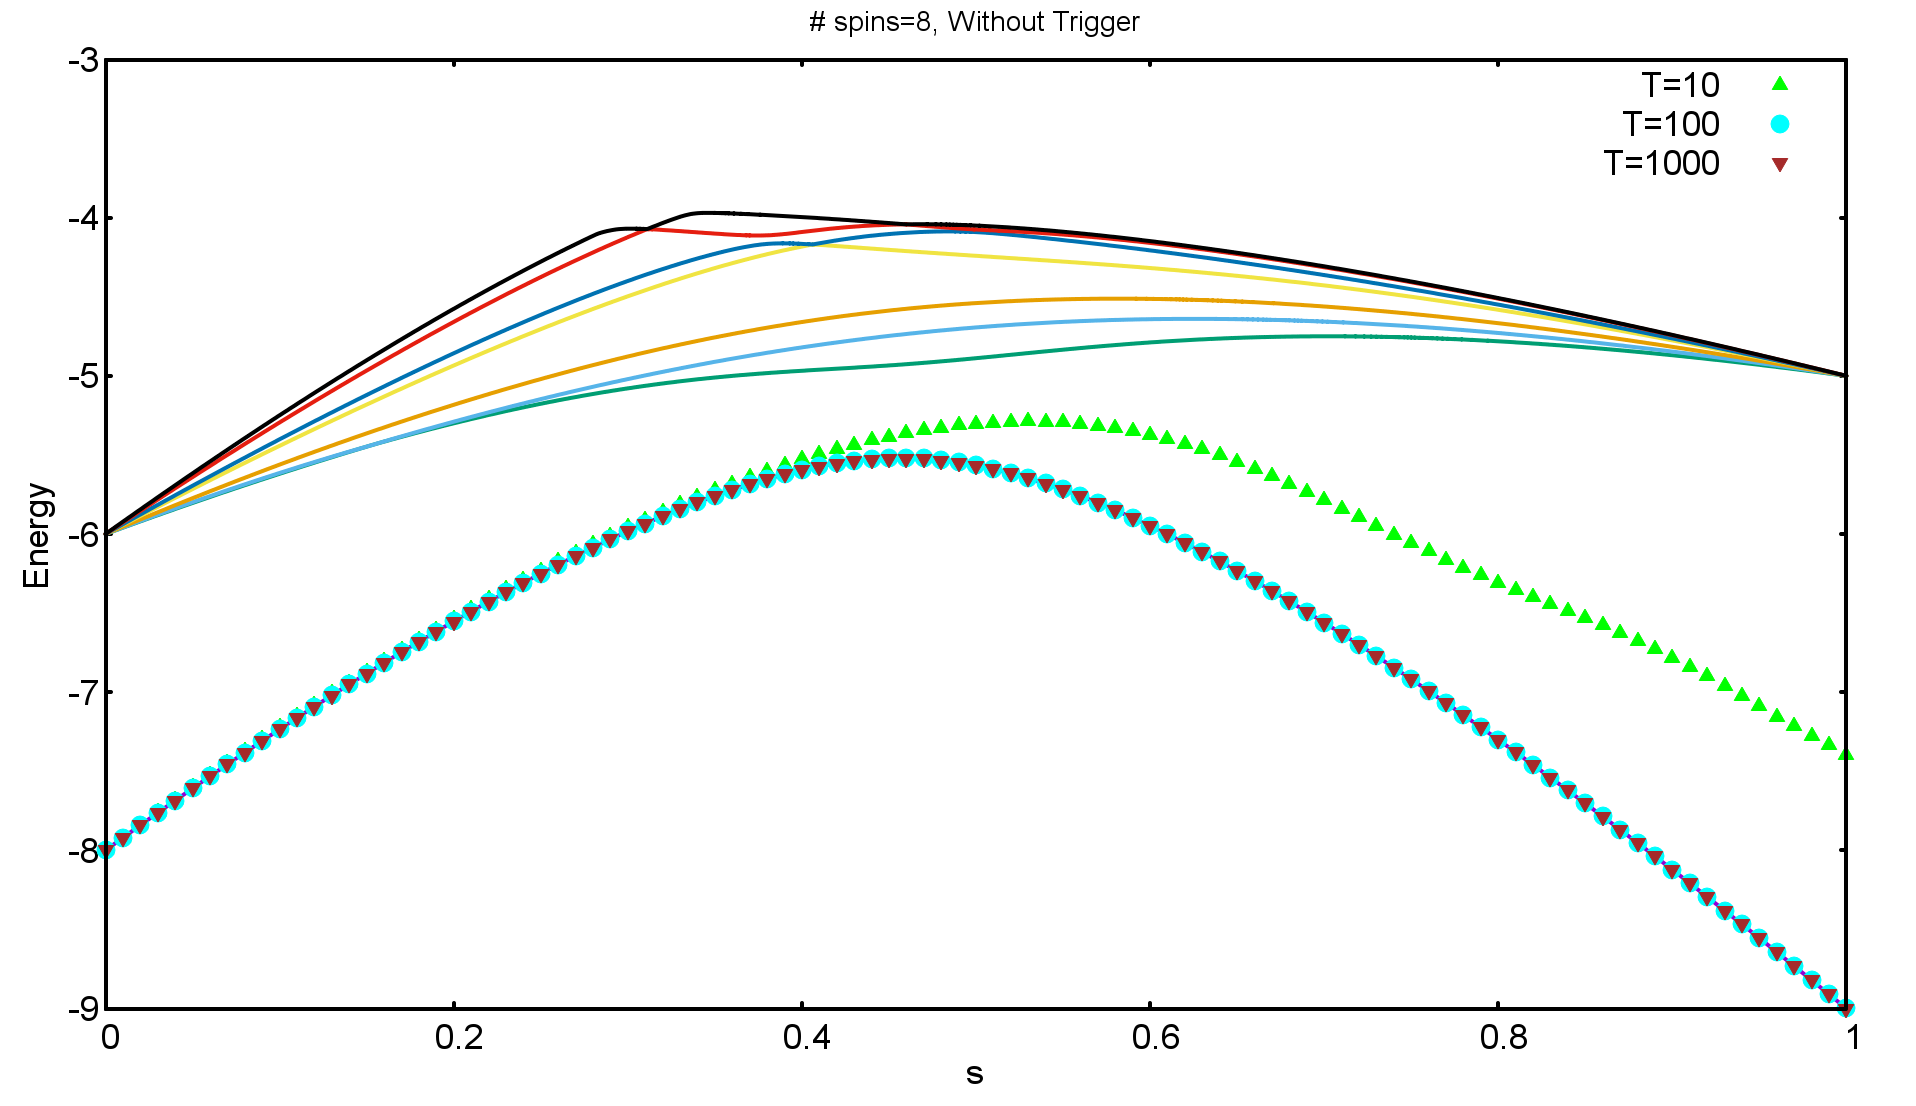
\includegraphics[scale=0.3]{98_s8_O.png}
\caption{The energy spectrum for the selected problem, with instantaneous energy values corresponding to three annealing times. For $T_A$=100, $p$ was found to be 0.999914, while $\Delta=0.587541$.}
\label{fig:o5}
\end{figure}
\begin{figure}[H]
\centering 
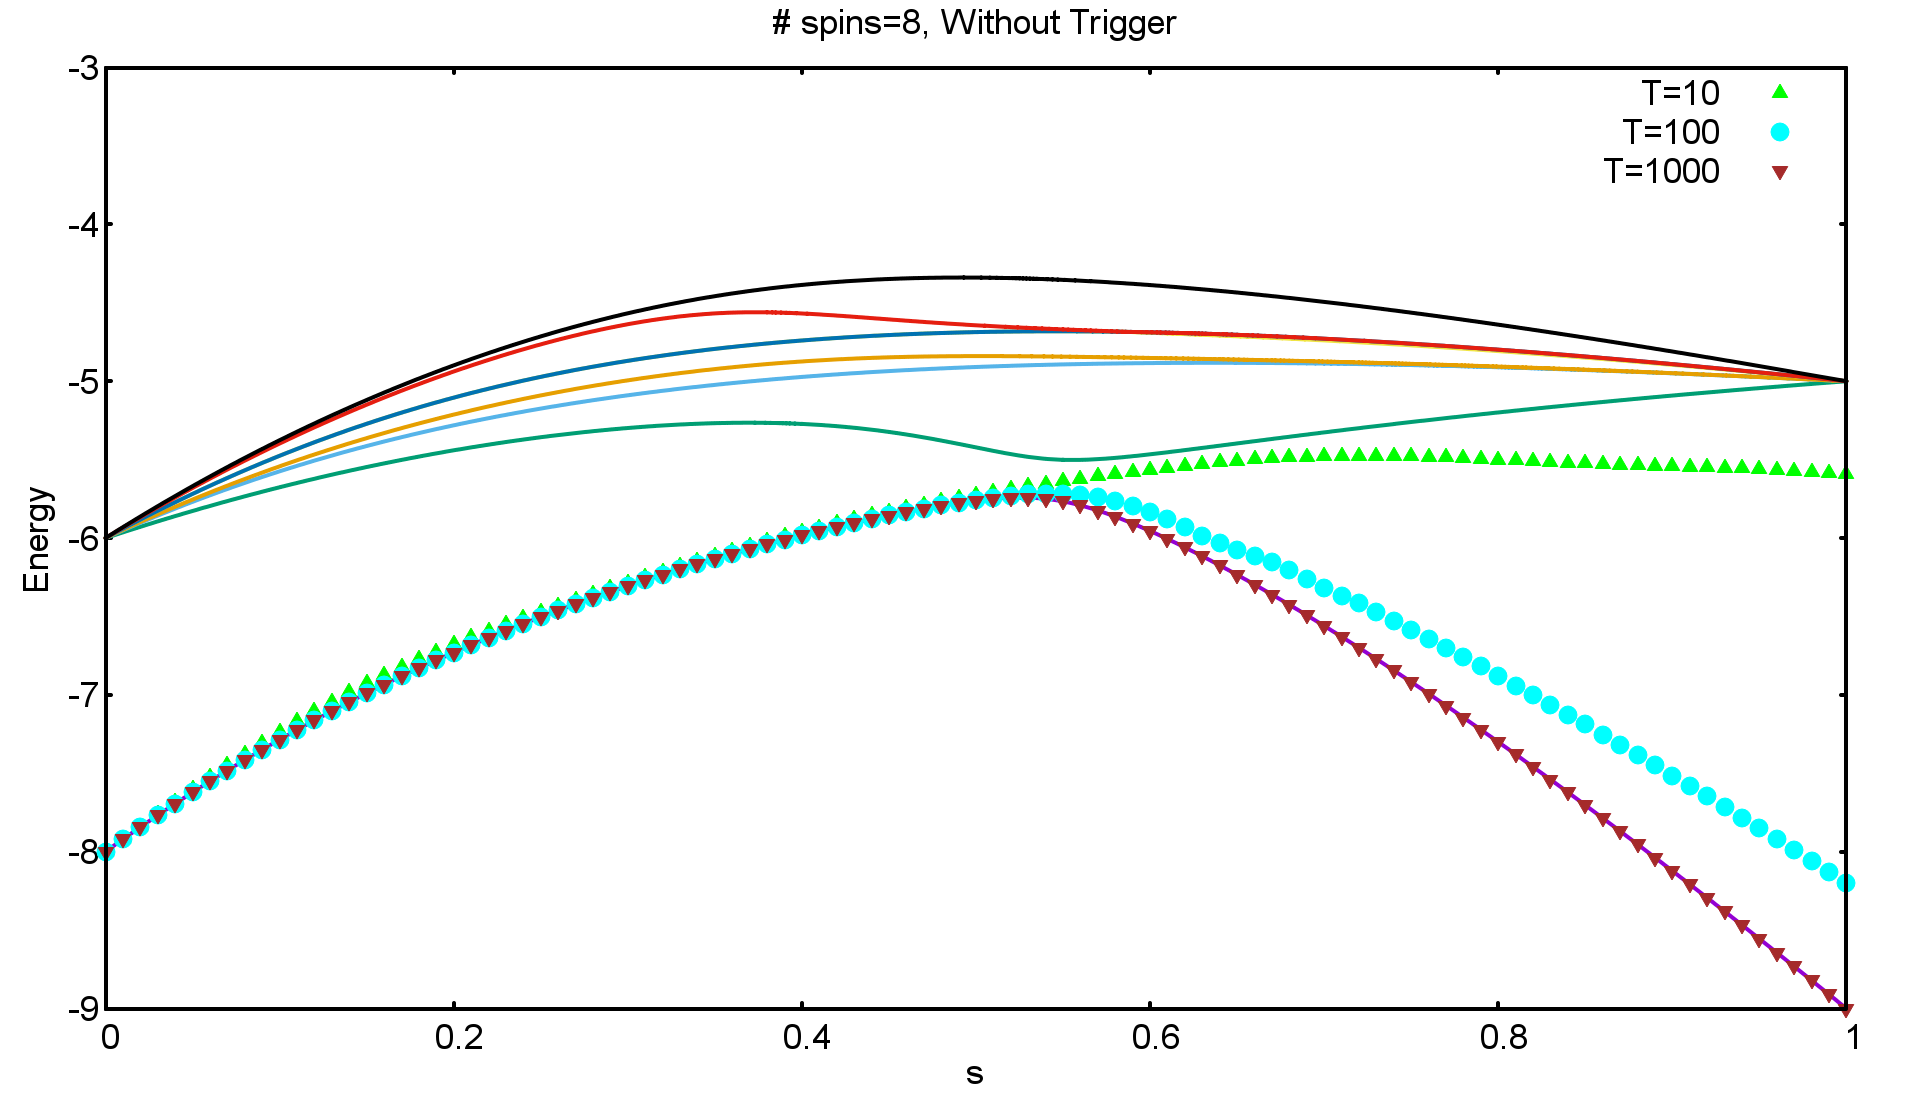
\includegraphics[scale=0.3]{79_s8_O.png}
\caption{The energy spectrum for the selected problem, with instantaneous energy values corresponding to three annealing times. For $T_A$=100, $p$ was found to be 0.799423, while $\Delta=0.322463.$}
\label{fig:o6}
\end{figure}
\begin{figure}[H]
\centering 
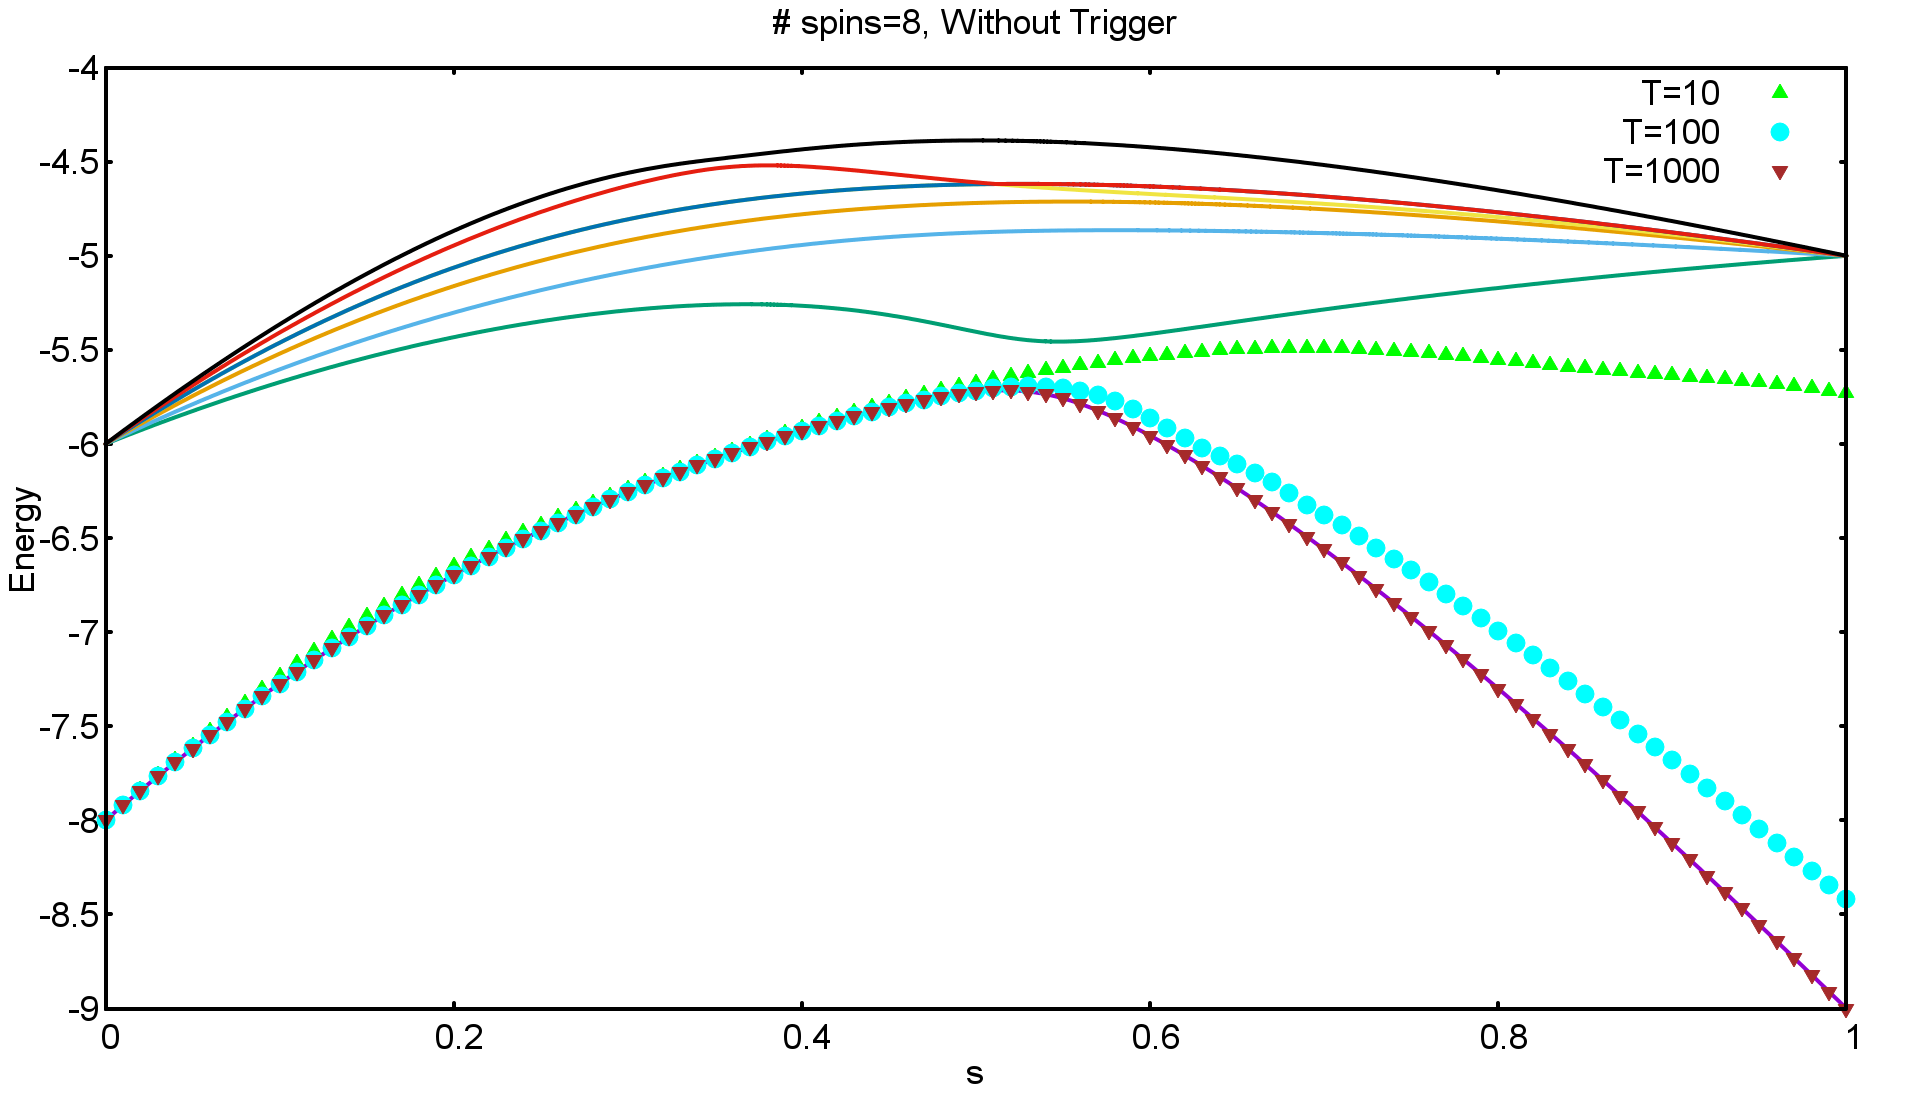
\includegraphics[scale=0.3]{59_s8_O.png}
\caption{The energy spectrum for the selected problem, with instantaneous energy values corresponding to three annealing times. For $T_A$=100, $p$ was found to be 0.854942, while $\Delta=0.472494.$}
\label{fig:o7}
\end{figure}
\newpage
To obtain a rough estimate of the spread of the difficulty of the problems in the set being considered here, figure (\ref{fig:o8}) shows a plot of the histogram of the probabilities of ending in the ground state of the problem Hamiltonian for an annealing time $T_A=100$. 
\begin{figure}[H]
\centering 
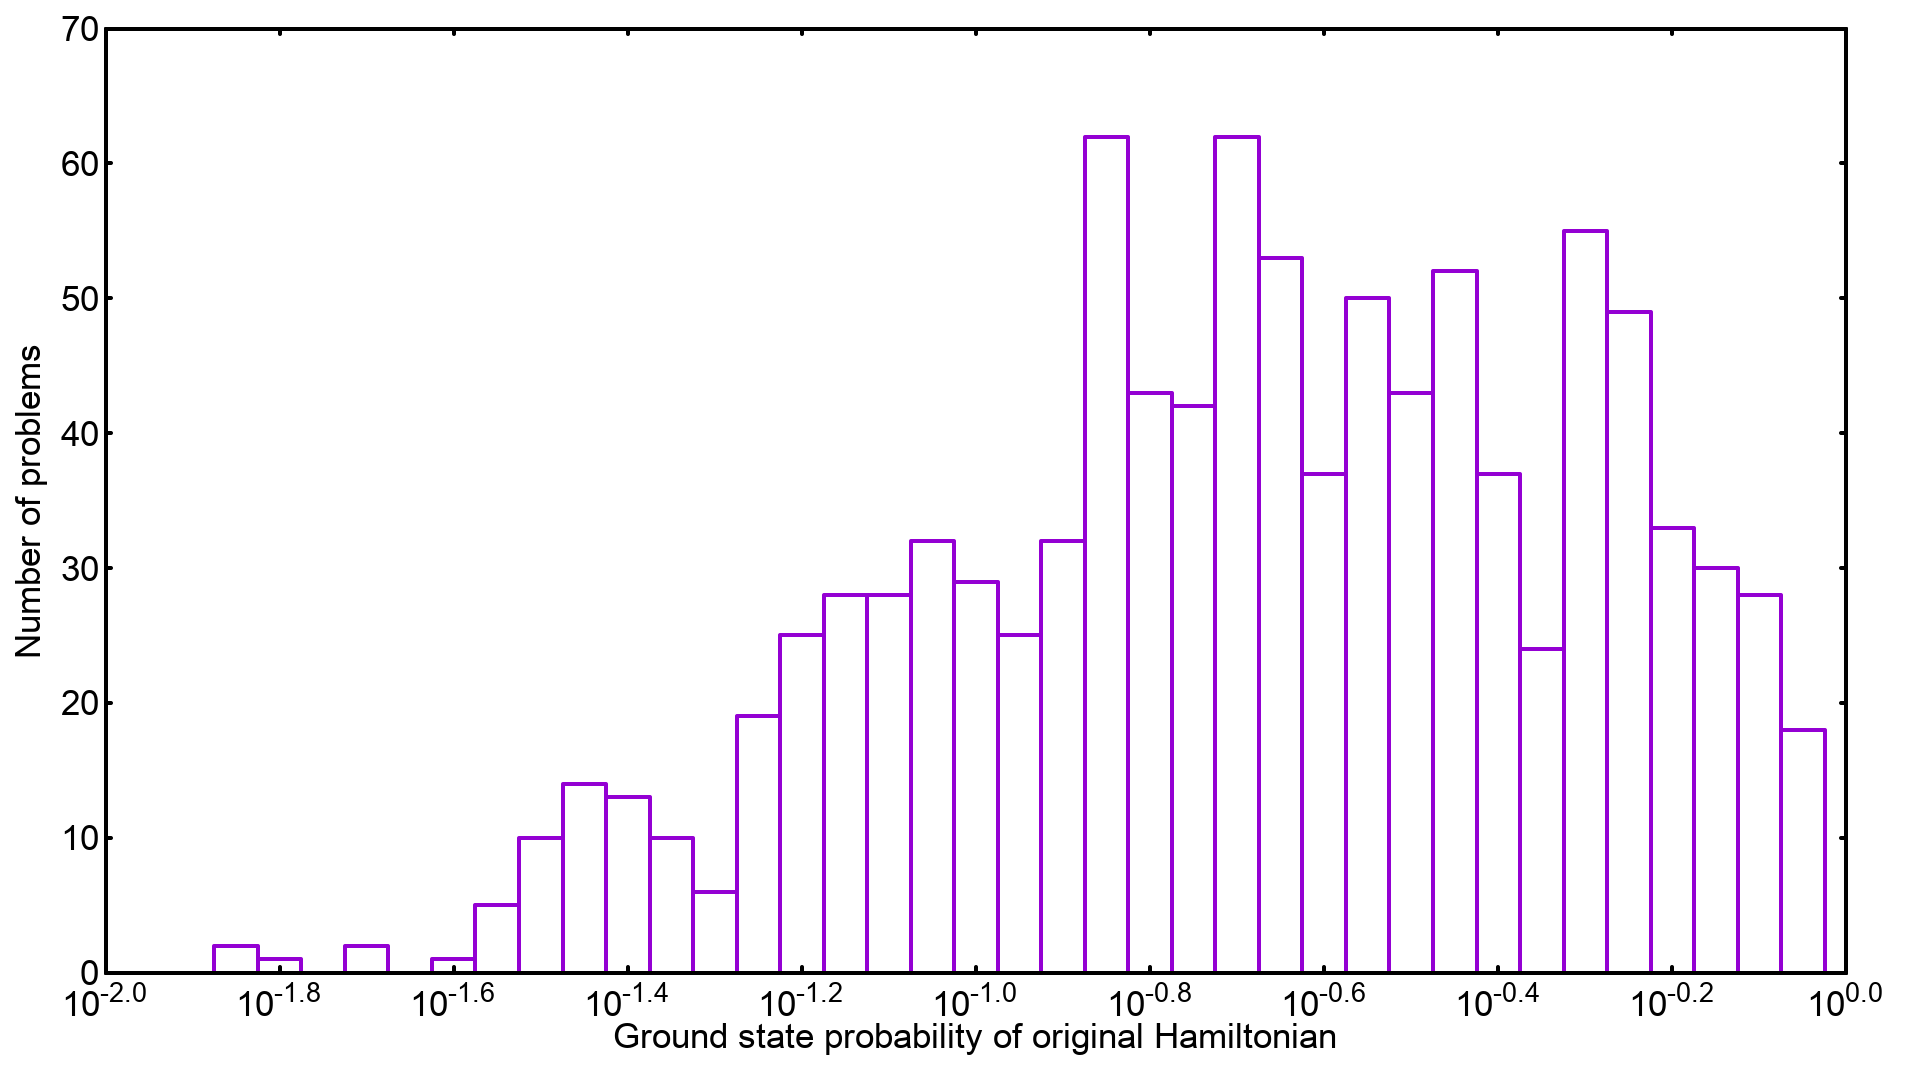
\includegraphics[scale=0.3]{O_s12_T100_g0.png}
\caption{Histogram for success probability of the Hamiltonians without any triggers for 1000 12-spin problems and $T_A$=100.}
\label{fig:o8}
\end{figure}
The similar histogram for 8-spin problems is shown in figure (\ref{fig:o9}) for an annealing time of $T_A$=10.
\begin{figure}[H]
\centering 
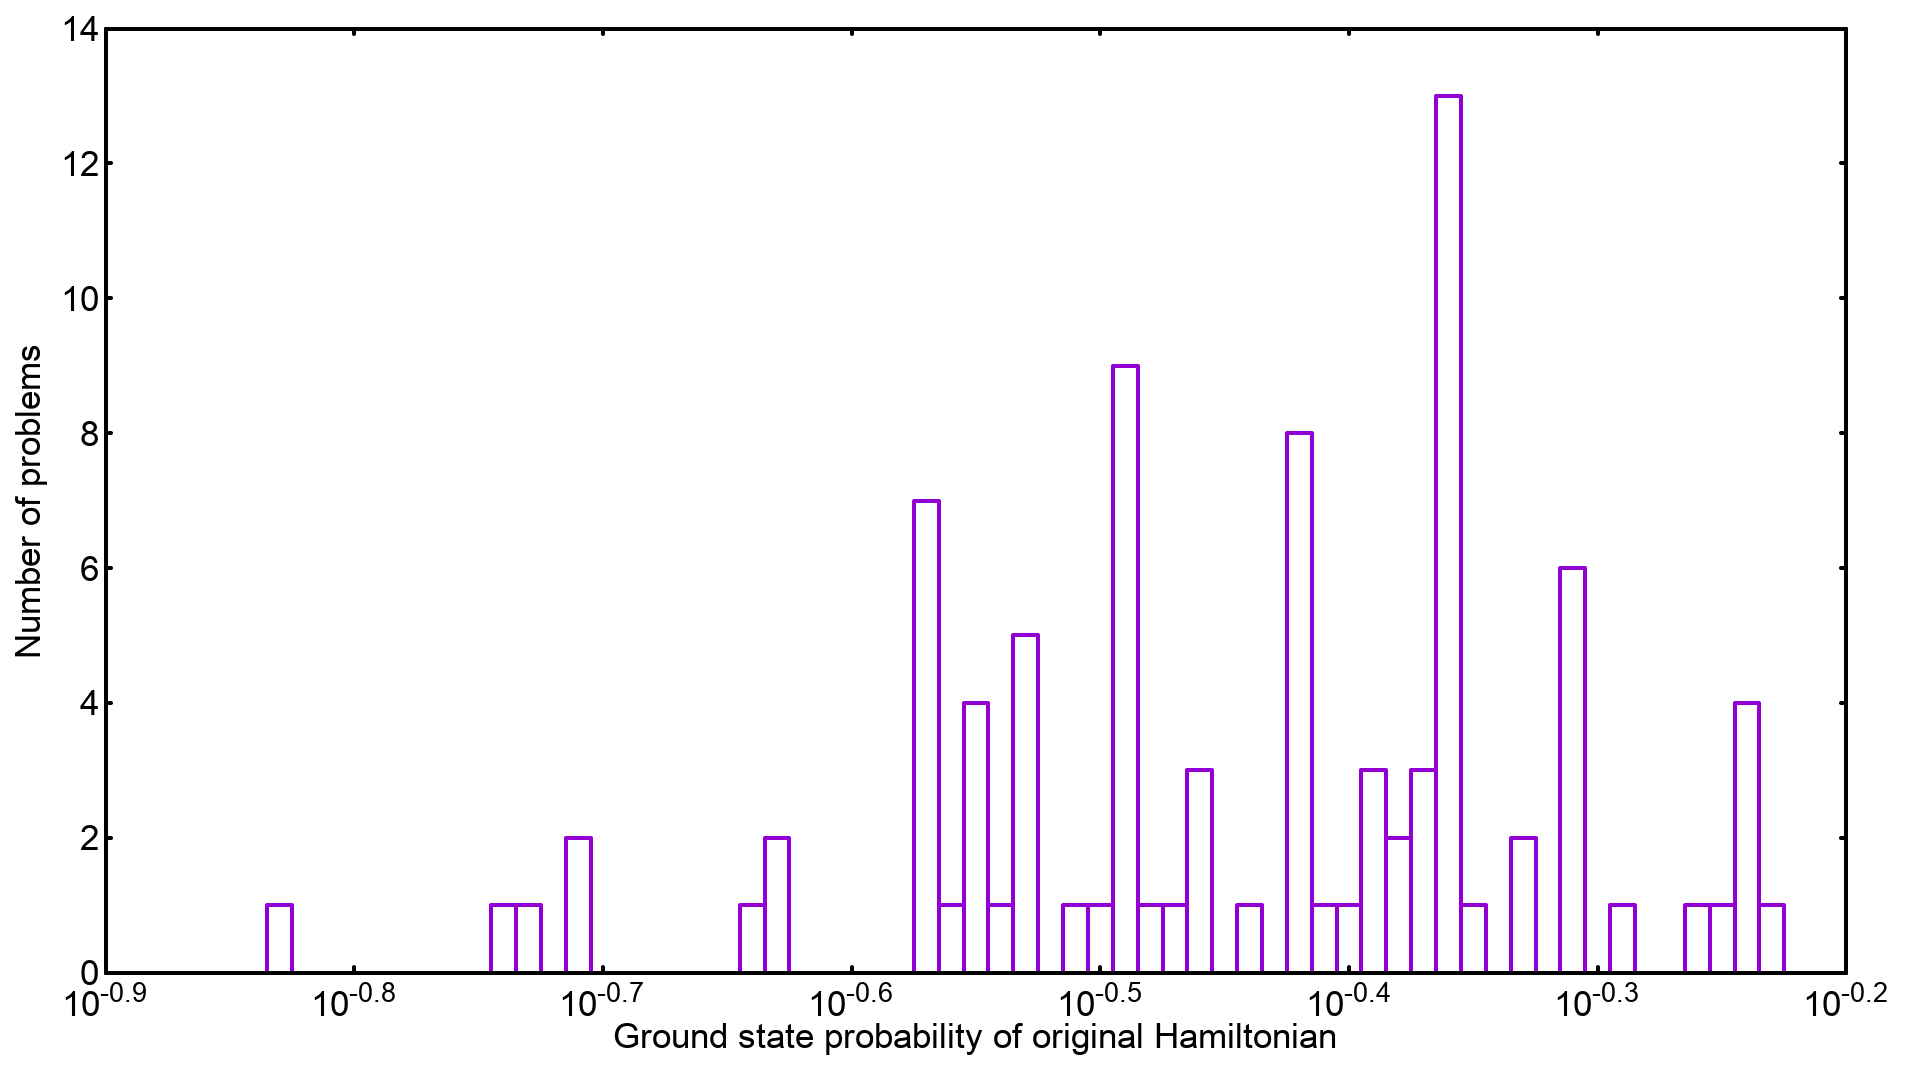
\includegraphics[scale=0.3]{O_s8_T10_g0.png}
\caption{Histogram for success probability of the Hamiltonians without any triggers for 91 8-spin problems and $T_A$=10.}
\label{fig:o9}
\end{figure}
Finally, to check if the sweeping from the initial Hamiltonian to the final Hamiltonian is adiabatic, the success probability of all the 12-spin problems have been plotted in figure (\ref{fig:o10}).
\begin{figure}[H]
\centering 
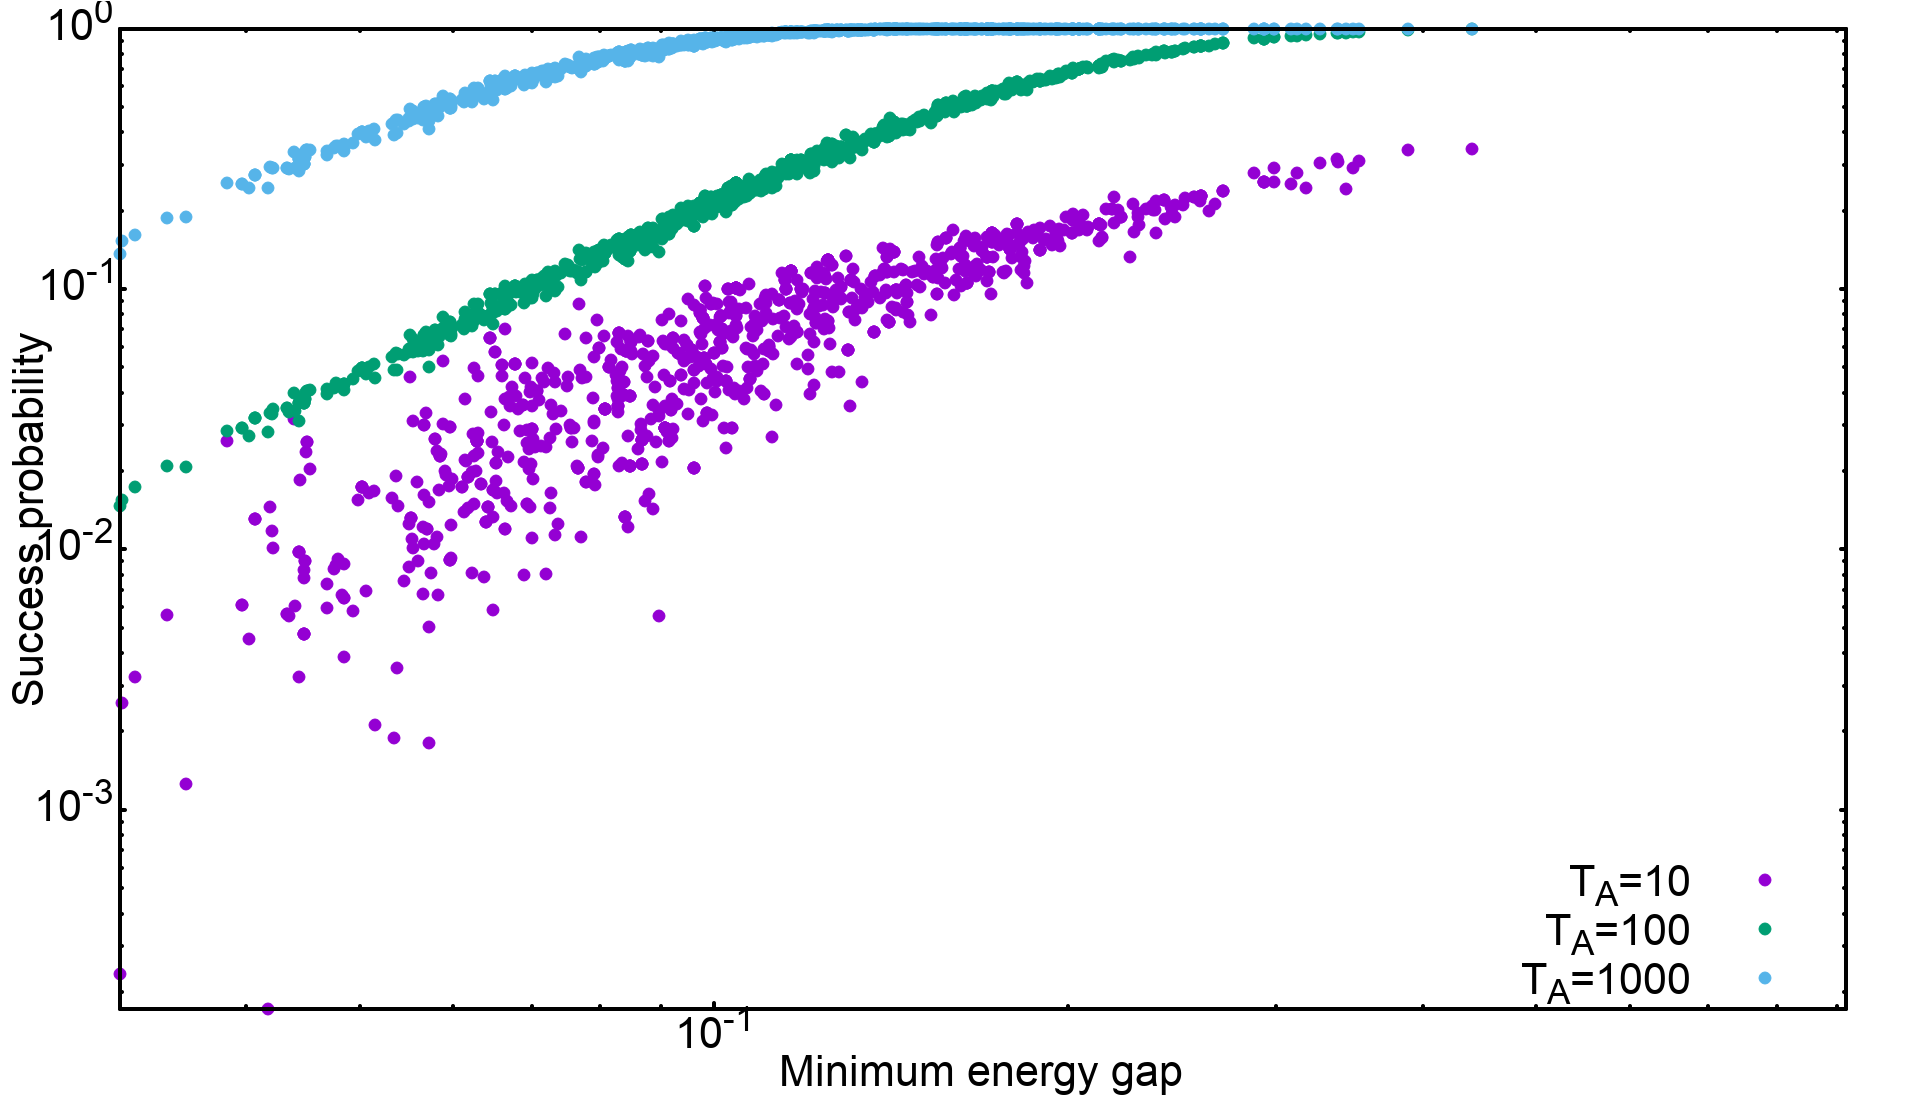
\includegraphics[scale=0.3]{GapVsSucc_s12_T10_100_1000.png}
\caption{Success probability Versus minimum energy gaps for all the 12-spin problems for annealing times of 10,100 and 1000.}
\label{fig:o10}
\end{figure}
From equation (\ref{eq:lz3}), the probability of ending in a state close to the ground state of the problem Hamiltonian increases exponentially with increasing the minimum energy gap between the ground and first excited state of the Hamiltonian, for fixed annealing time. Since different problems, corresponding to different minimum energy gaps are found to have an exponential relation in the success probability and the minimum energy gaps, the annealing is indeed adiabatic. However, for small annealing times, the scattering in the plot increases. 

A similar plot for 8-spin problems is shown in figure (\ref{fig:o11}).
\begin{figure}[H]
\centering 
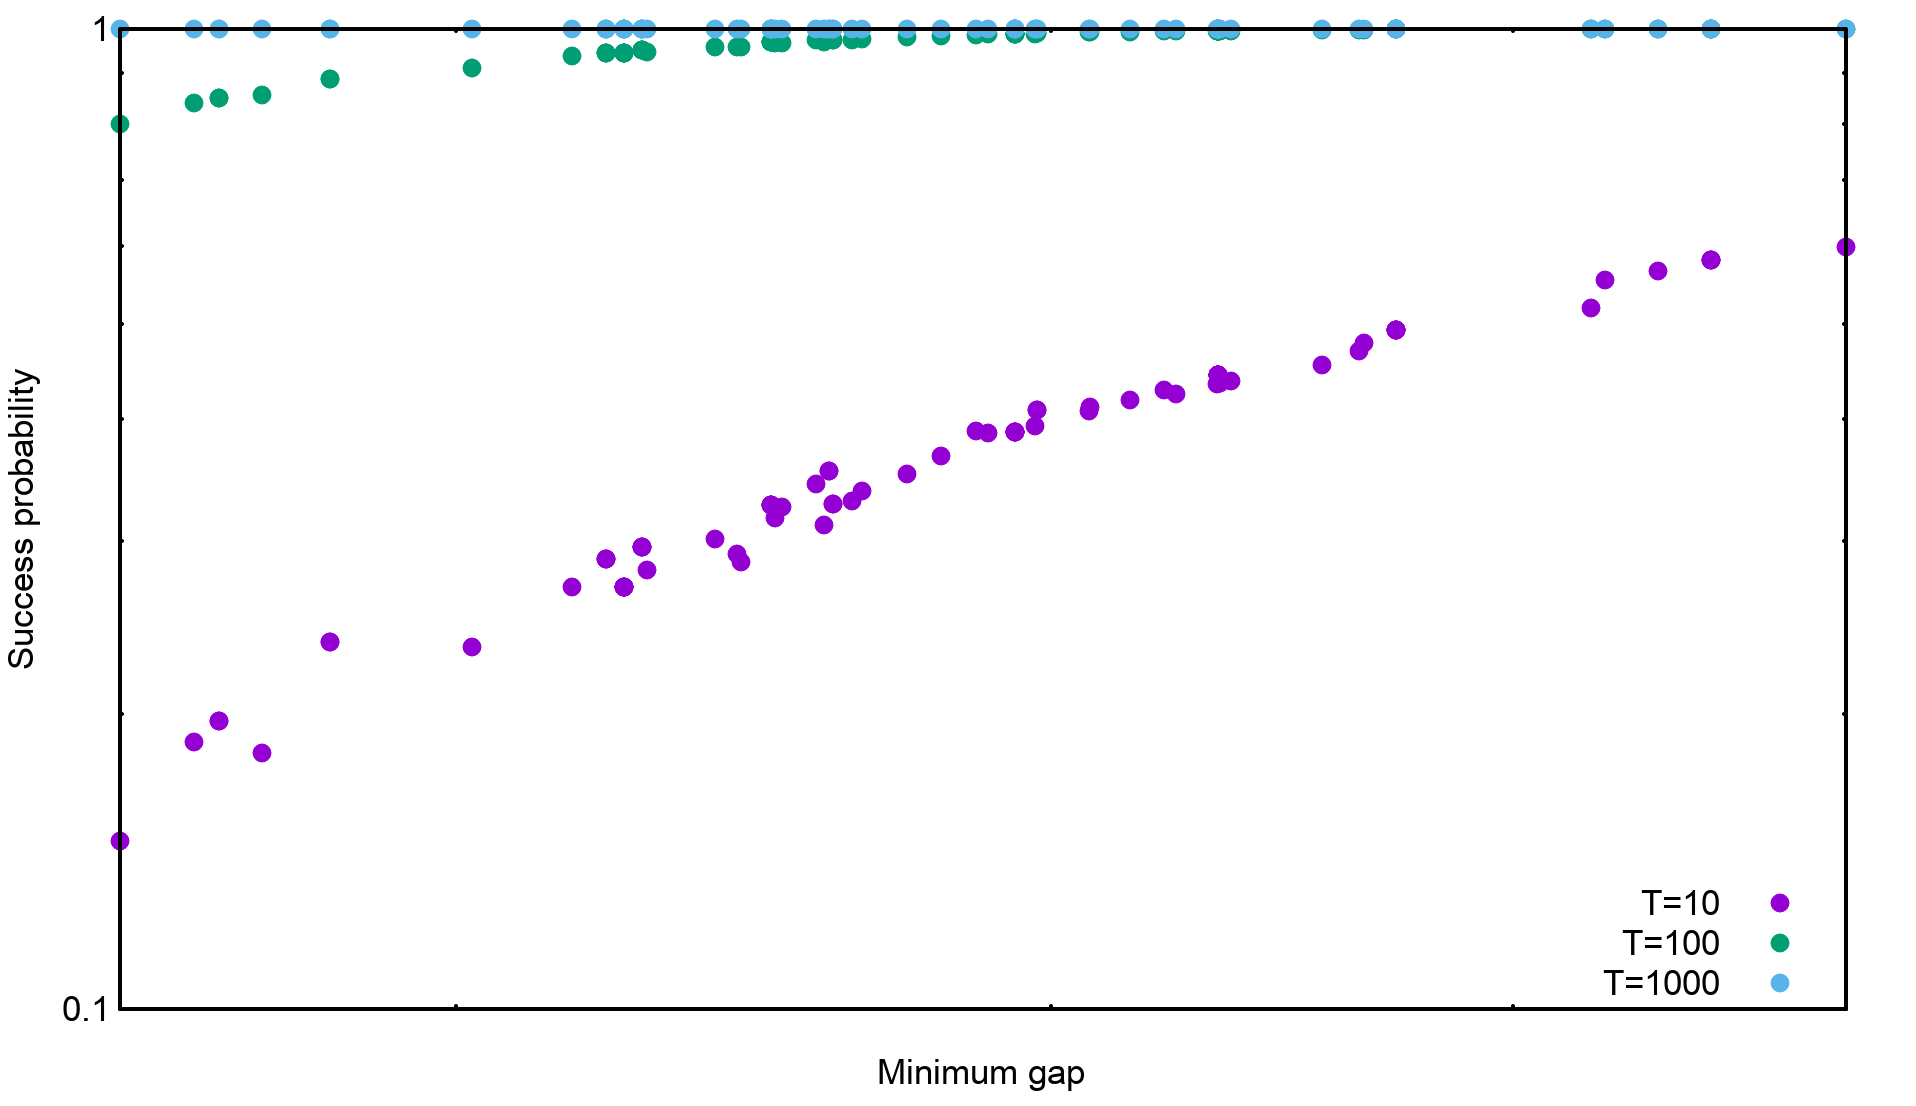
\includegraphics[scale=0.3]{GapVsSucc_s8_T10_100_1000.png}
\caption{Success probability Versus minimum energy gaps for all the 8-spin problems for annealing times of 10,100 and 1000.}
\label{fig:o11}
\end{figure}
\end{document}